\documentclass{article}
\usepackage[utf8]{inputenc}

\usepackage{graphicx}

\newcommand{\coursecode}{CS311}
\newcommand{\coursename}{\emph{Automata Theory and Formal languages}}


\title{Homework Assignment 1 \hfill\\
\small
\coursecode, \coursename}


\author{Joshua F. Clemente \hfill\\
        20-00435 \hfill\\
        20-00435@g.batstate-u.edu.ph \hfill\\
}
\date{December 2 2022}

\begin{document}

\maketitle

\section{Can you compute the NOT's of 3 input variable, using as many AND/OR gates as you like but only 2 NOT gates?}

    With the available logic gates, it is possible. It is accomplished by using inverter outputs as input for another input. stating that the NOT gate will have an effect on all three inputs (A, B, and C). According to the diagram, the NOT gate will have an effect on the second NOT gate or act as its input. The objective is to design a circuit whose output matches the OR gate, serving as the circuit's final gate. This indicates that having the output of the three connected to one another creates a natural inverter (NOT) through its relationships with the use of only two NOT.

    
    \begin{figure}[h!]
    \centering
    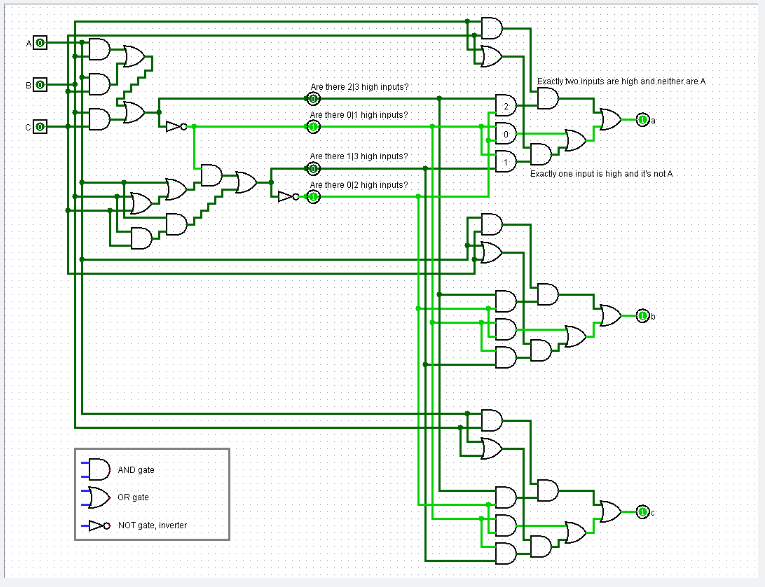
\includegraphics[height = 7cm, width = 11cm]{sheeesh.png}
    \end{figure}

    References:

    https://electronics.stackexchange.com/questions/98308/can-i-get-the-not-of-3-inputs-using-as-many-and-or-gates-but-only-2-not-gates  \hfill\\
    \hfill\\ https://puzzling.stackexchange.com/questions/9438/invert-three-inputs-with-two-not-gates \hfill\\

\end{document}
